%! Author = Filippo Vissani
%! Date = 08/02/24
% !TeX root = ../thesis-main.tex

%----------------------------------------------------------------------------------------
\chapter{Analysis}
\label{chap:analysis}
%----------------------------------------------------------------------------------------
\section{State of the Art}

\subsection{Protelis}

Protelis~\cite{Pianini2015} is based on field calculus and is closely related to Proto~\cite{Beal2006}. It inherits spatial computing features from the field calculus, which provides universality, consistency, and self-stabilization properties. However, Protelis improves over Proto by offering a richer API through Java integration, support for code mobility through first-order functions, and a syntax inspired by C-family languages.

The syntax of Protelis (\Cref{fig:protelis-syntax}) is presented in abstract form. It uses meta-variables to represent names of user-defined functions (\texttt{f}), variables and function arguments (\texttt{x}), literal values (l), built-in functions and operators (b), Java method names (\texttt{m}), and aliases of static Java methods (\texttt{\#a}). The syntax employs conventions like comma-separated lists and semi-colon separators for sequences of elements.

Protelis adopts a familiar C- or Java-like syntax, making it more accessible and reducing barriers to adoption. Despite its syntactic similarity to imperative languages, Protelis is purely functional. Programs consist of a sequence of function definitions, followed by a main block of statements. Functions are defined with curly brackets and can contain sequences of statements or expressions. Each statement is an expression to be evaluated (\texttt{e}), possibly in the context of the creation of a new variable (\texttt{let x = e}) or a re-assignment (\texttt{x = e}).

\begin{figure}
    \centering
    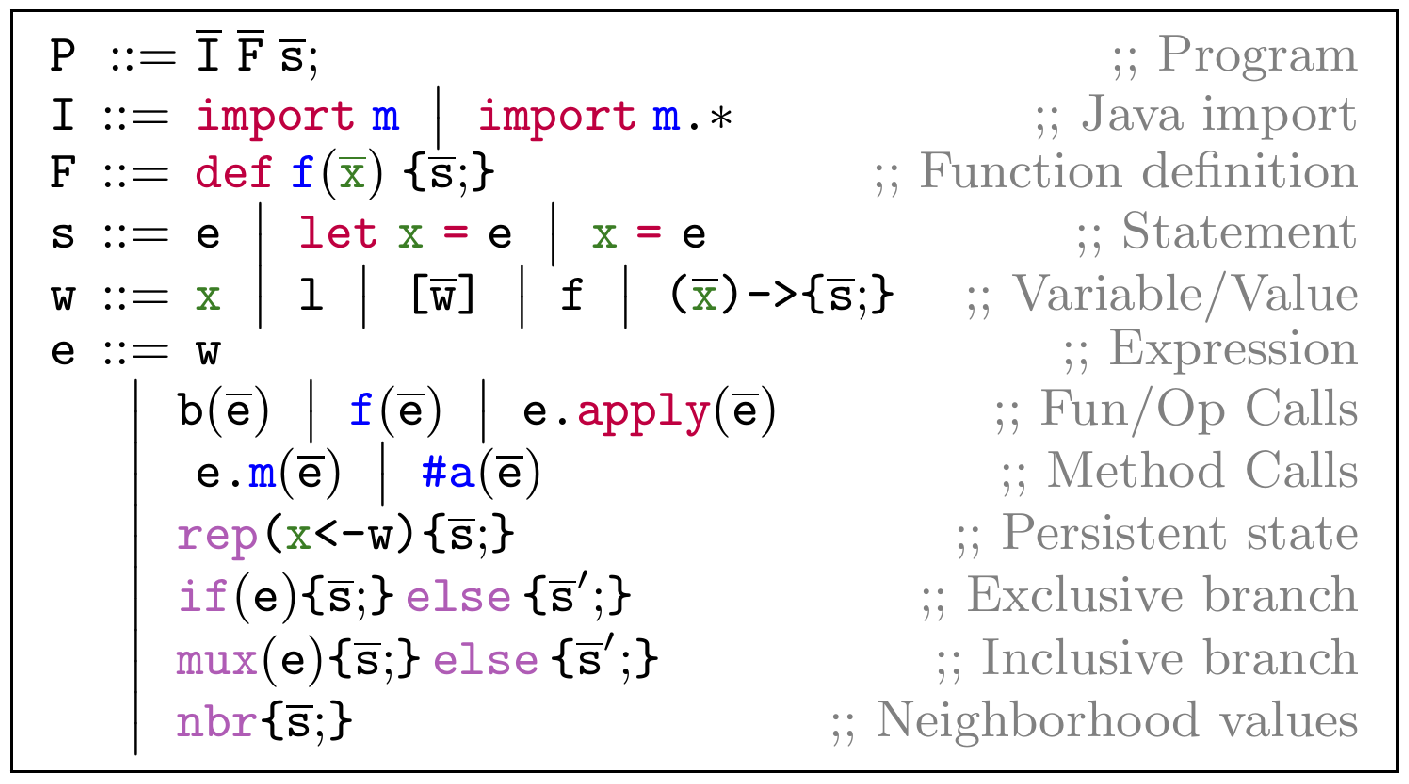
\includegraphics[width=\linewidth]{figures/protelis-syntax.png}
    \caption{Protelis abstract syntax}
    \label{fig:protelis-syntax}
\end{figure}

\subsubsection{Example: Rendezvous at a Mass Event}

In large public events, it can be challenging to meet with companions due to crowded areas, inaccessible rendezvous points, or difficulty in accessing cloud-based services.

Utilizing peer-to-peer geometric calculations across a network of devices to compute a \textit{rendezvous}\footnote{A meeting at an agreed time and place.} route is the proposed solution to the problem. The solution is demonstrated in a simulated city center environment (\Cref{fig:protelis-example-map}), using London as an example, with devices distributed randomly across the city streets. Each device has a communication range, and the goal is for two individuals (represented by their devices) to meet at a specific location.

The implementation (\Cref{lst:protelis-example}) involves injecting the environment of the devices with properties representing their owners (e.g., "Alice" and "Bob"). The algorithm measures the distance to one of the participants, creates a potential field, and builds an optimal path from the other participant, descending the distance potential field to reach the first participant at zero distance. The algorithm utilizes two main functions: \texttt{distanceTo} and \texttt{descend}. \texttt{distanceTo} measures the distance to one of the participants. Given a device and a potential field, \texttt{descend} builds a path of devices connecting the device with the source of the potential field. The algorithm elegantly compresses the entire process into a few lines of code, utilizing the \texttt{nbr} operator to exchange required information without explicitly declaring any communication protocol.

As \Cref{fig:protelis-example-map} shows, the simulation rapidly identifies a chain of devices (represented by red dots) that marks a sequence of waypoints for both device owners to walk and meet in the middle. The algorithm dynamically adjusts the path if one of the device owners moves in a different direction, ensuring it continues to recommend the best path for rendezvous.

\lstinputlisting[float,label={lst:protelis-example},caption=Rendezvous implementation in Protelis]{listings/protelis-example.txt}

\begin{figure}
    \centering
    \begin{subfigure}[b]{.49\textwidth}
        \centering
        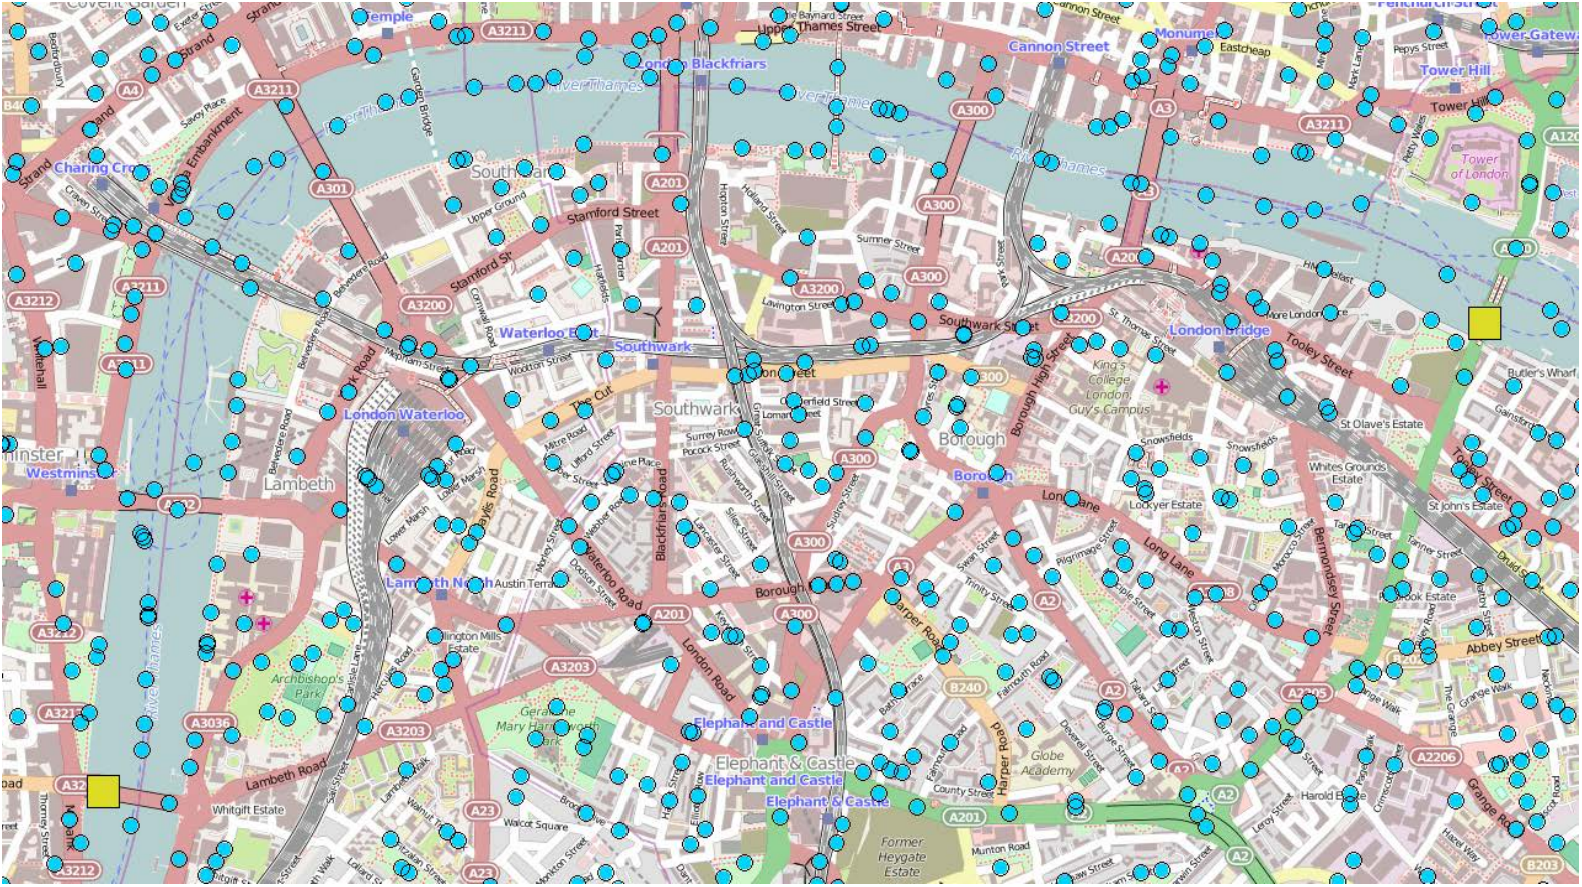
\includegraphics[width=\textwidth]{figures/protelis-example-a.png}
        \caption{Initial configuration.}
        \label{fig:protelis-example-a}
    \end{subfigure}
    \hfill
    \begin{subfigure}[b]{.49\textwidth}
        \centering
        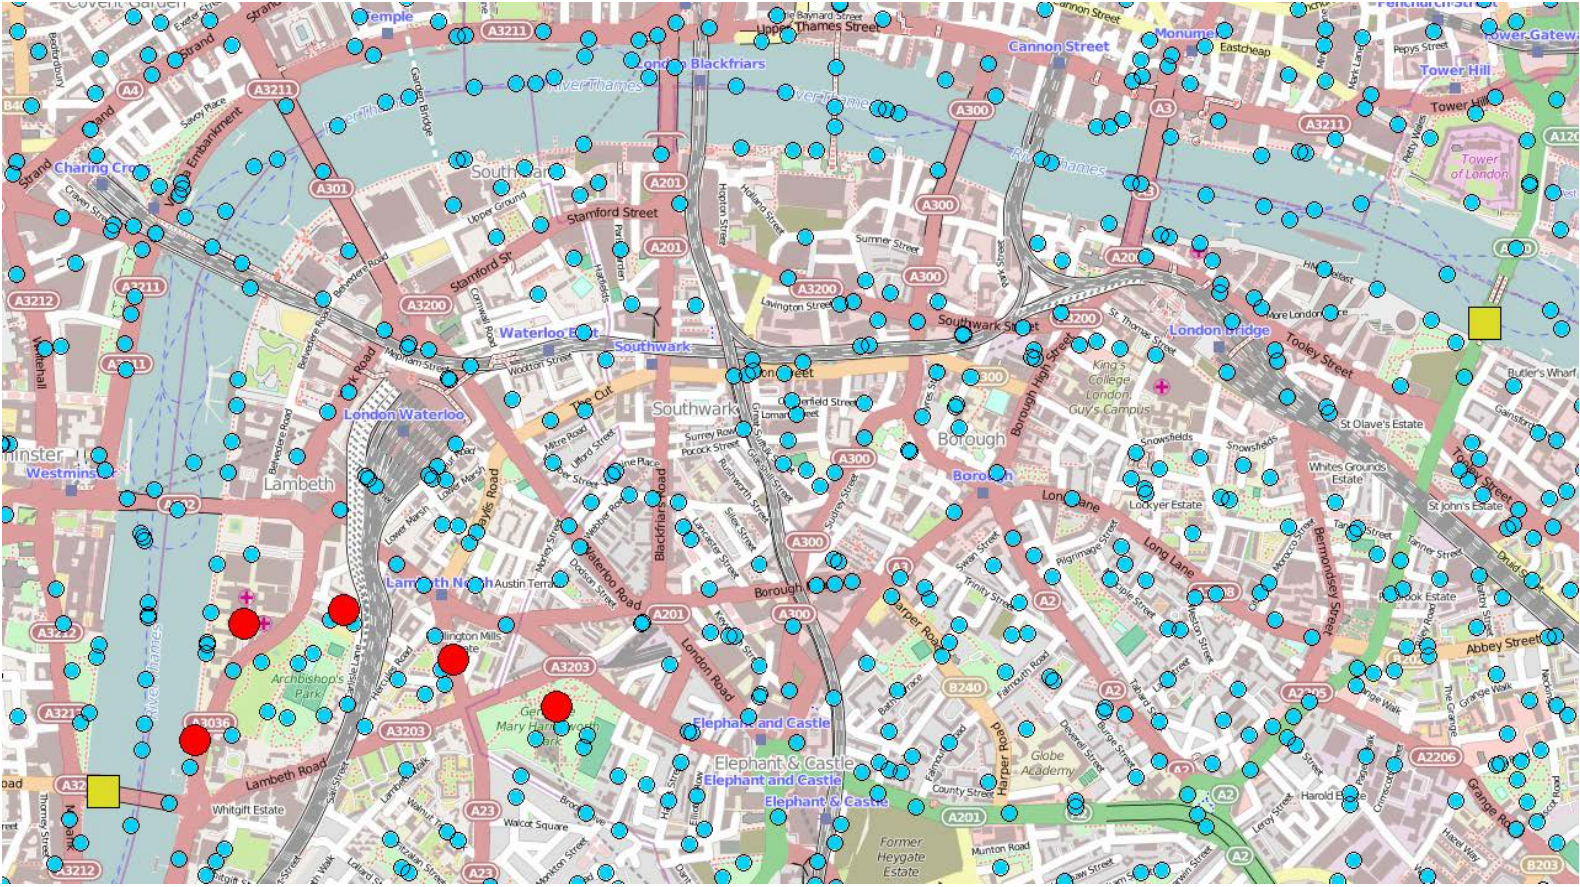
\includegraphics[width=\textwidth]{figures/protelis-example-b.png}
        \caption{Path begins to form.}
        \label{fig:protelis-example-b}
    \end{subfigure}
    \hfill
    \begin{subfigure}[b]{.49\textwidth}
        \centering
        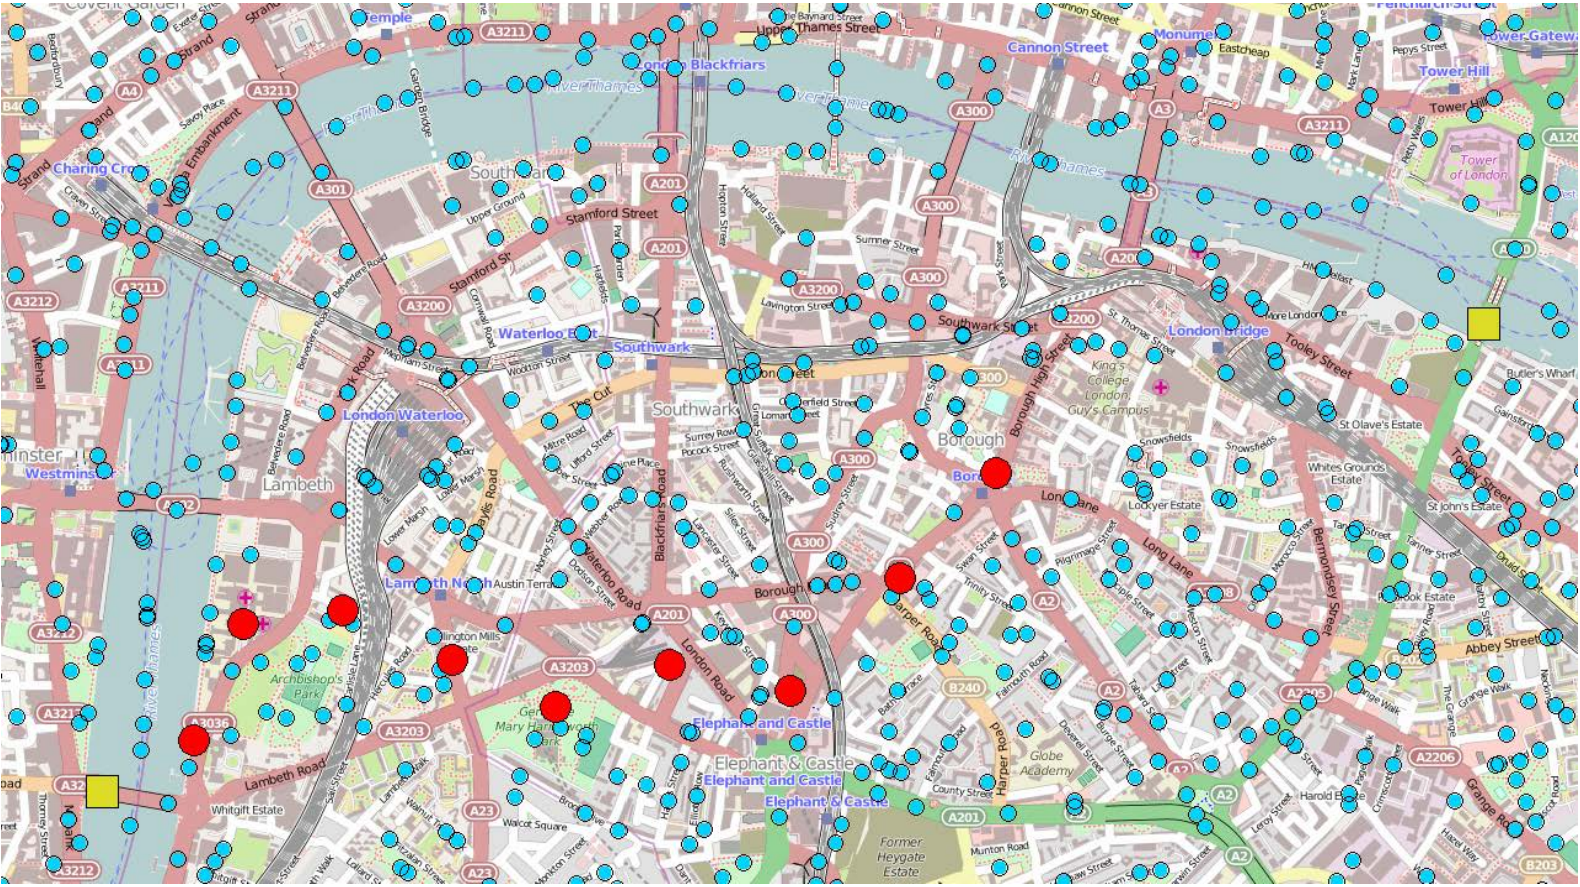
\includegraphics[width=\textwidth]{figures/protelis-example-c.png}
        \caption{Path continues to extend.}
        \label{fig:protelis-example-c}
    \end{subfigure}
    \hfill
    \begin{subfigure}[b]{.49\textwidth}
        \centering
        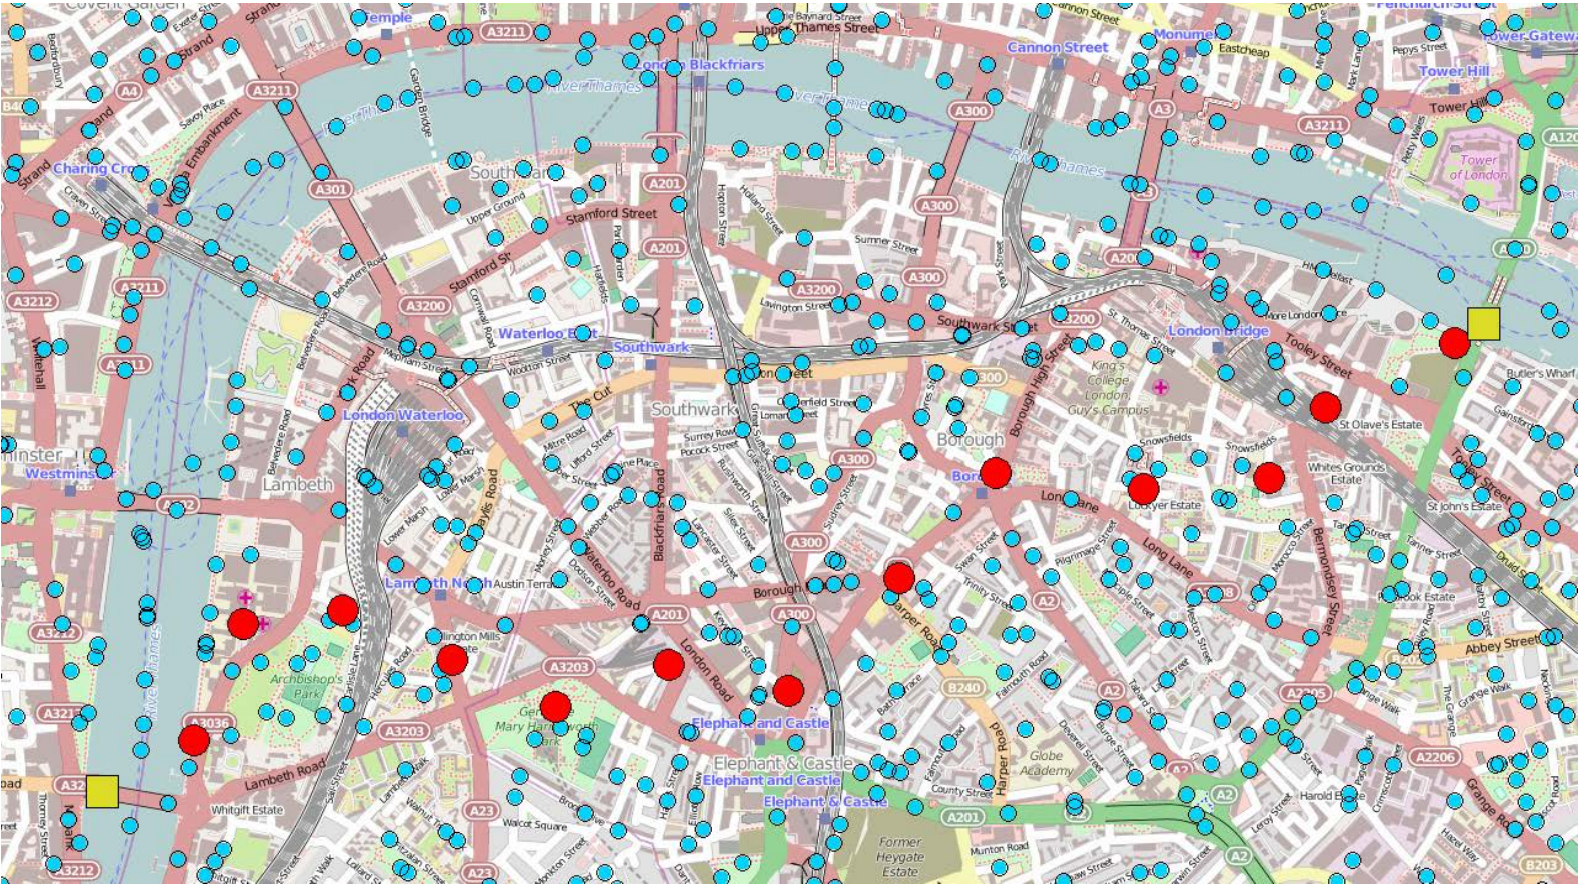
\includegraphics[width=\textwidth]{figures/protelis-example-d.png}
        \caption{Path computation complete.}
        \label{fig:protelis-example-d}
    \end{subfigure}
    \caption{Example of computing a rendezvous route for two people in a crowded urban environment.}
    \label{fig:protelis-example-map}
\end{figure}


\subsection{ScaFi}

\subsection{FCPP}

\subsection{Collektive}

\subsection{FRASP}

As said in \Cref{subsection:reactive-and-proactive-models}, aggregate computing makes use of a round-based execution model, that can be defined as \textit{proactive}. This approach is simple to reason about but limited in terms of flexibility in scheduling and management of sub-activities (and response to contextual changes). In~\cite{Casadei2023} is proposed a reactive self-organization programming approach, called FRASP, that enables the decoupling of the program logic from the scheduling of its sub-activities. This model maintains the same expressiveness and benefits of aggregate programming while enabling significant improvements in terms of scheduling controllability, flexibility in the sensing/actuation model, and execution efficiency.

\subsubsection{Reactive Model}
FRASP is based on the reactive functional programming (FRP) paradigm and considers \textit{continuous time}, $Time$ = $\{ t \in \mathbb{R} \, | \, t \geq 0 \}$. Time-varying values are called \textit{cells} and may be conceptually modeled by generic functions of type $Cell$ $a$: $Time \rightarrow a$. Then, \textit{streams} are discrete-time values and may be modeled by generic functions of type $Stream$ $a$: $[Time] \rightarrow [a]$, namely, mapping a sequence of (increasing) sample times to a sequence of corresponding values. While cells model state, streams model state changes.

\subsubsection{Abstractions and Primitives}

One of the main differences between the proactive and reactive models is that the latter allows the self-organizing collective computation to be expressed as a graph of reactive sub-computations. Each sub-computation is called \textit{flow} and represents it programmatically through type \texttt{Flow[T]}, where \texttt{T} is the type of the output of the wrapped computation. A \texttt{Flow} is essentially a function that takes a \texttt{Context} and returns a cell of \texttt{Export}s, possibly depending on the exports of other \texttt{Flow}s, recursively.

The details of the syntax and semantics of FRASP are discussed in detail in Section III of~\cite{Casadei2023} while in this section they are presented in a simplified manner:

\begin{itemize}
    \item \texttt{constant(e)} returns a constant flow that always evaluates to the argument that has been passed;
    \item \texttt{sensor(name)} returns the flow of values produced by the sensor with the given \texttt{name};
    \item \texttt{mid()} returns the constant flow of the device ID;
    \item \texttt{mux(c)\{t\}\{e\}} is an expression that returns a flow with the same output of flow \texttt{t} when the Boolean flow \texttt{c} is true and the output of flow \texttt{e} when \texttt{c} is false;
    \item \texttt{nbr(f)} handles communication with neighbors in both directions at once, it takes a flow \texttt{f} as a parameter;
    \item \texttt{branch(c)\{t\}\{e\}} evaluates and returns the value of expression \texttt{t} when \texttt{c} evaluates to true. This enables a form of distributed branching, where devices that happen to execute \texttt{t} will not interact with those that executed \texttt{e} (and vice versa);
    \item \texttt{loop(init,ft)} evolves a piece of state (initially, \texttt{init}) by applying function \texttt{ft} mapping the previous state's flow to the next state's flow.
\end{itemize}

\subsubsection{A Paradigmatic Example}

A \textit{(self-healing) gradient} is a distributed behavior that self-stabilizes, in each device of the distributed system, to a value denoting its minimum distance from the closest source node (for instance, computed by summing the neighbor-to-neighbor distances along the shortest path to the source), adapting to changes in the source set and distances. By following the neighbors of maximum decrease (resp. increase) of the gradient value, i.e., by descending (resp. ascending) the gradient, it is possible to implement efficient hop-by-hop information flows, that can be useful for data propagation and collection. \Cref{lst:gradient.scala} provides a representation of a gradient. The function takes the Boolean \texttt{src} flow as input, denoting whether the executing node is the source of the gradient or not. The external \texttt{loop} is used to progressively evolve the current gradient value \texttt{distance} starting from an infinite value (as, initially, devices do not know whether a source is reachable). Internally to the loop, \texttt{mux} is used to select one of two values: if the node is a source, then its gradient value is \texttt{0} (base case); otherwise, the gradient should be the minimum value among the neighbors' gradient values augmented by the distance (\texttt{nbrRange}) from that very neighbor. Construct \texttt{liftTwice} is used to combine (using the sum: \_+\_) the two flows \texttt{nbrRange} (distances to neighbors) and \texttt{nbr(distance)} (neighbors' gradient values).

\lstinputlisting[label={lst:gradient.scala},language=scala,caption=Gradient implementation in FRASP]{listings/gradient.scala}

The reactive dataflow graph in \Cref{fig:gradient-dependencies} corresponds to \Cref{lst:gradient.scala}. \Cref{fig:gradient-dependencies} provides the local view of the computation for a single node (where the layers denote different semantic kinds of dependencies), whereas \Cref{fig:gradient-dependencies-distributed} shows the distributed dependency graph. The arrows denote dependencies. The dashed arrows denote dependencies based on platform-level scheduling and node interaction; for instance, a red block depends on changes corresponding to neighbors' red blocks and is communicated via message passing.

\begin{figure}
    \centering
    \begin{subfigure}[b]{\textwidth}
        \centering
        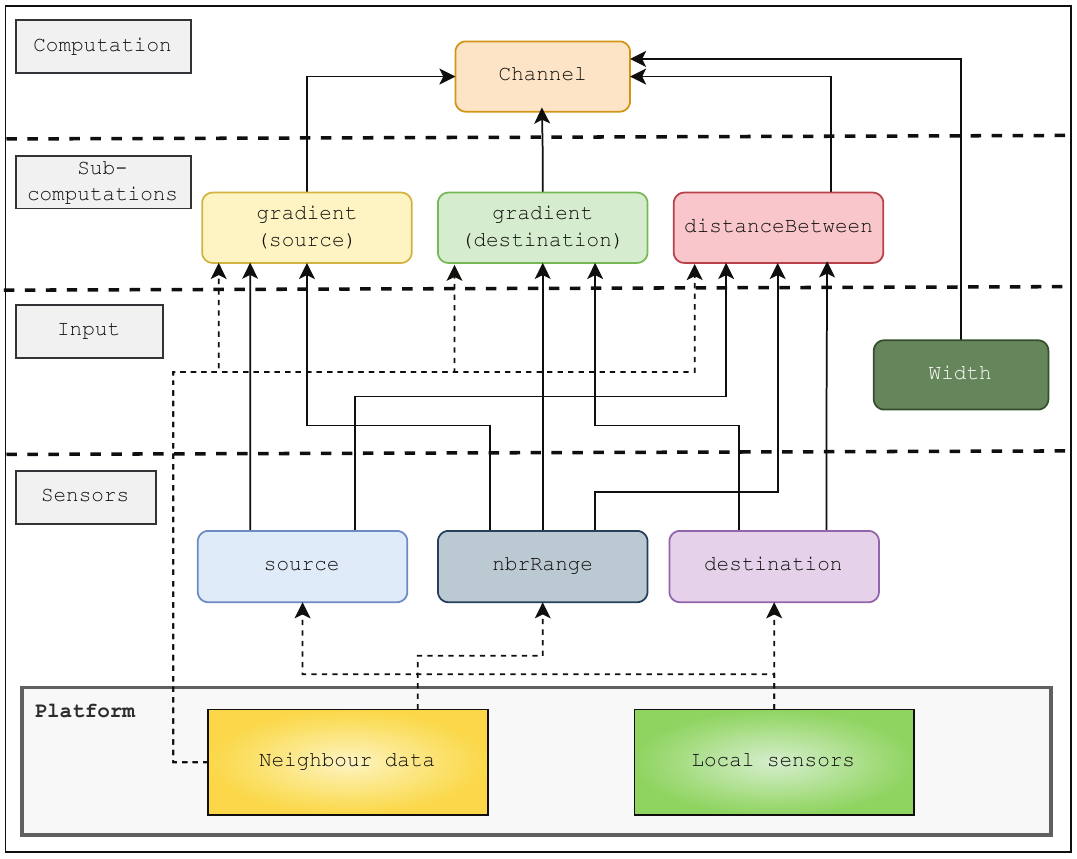
\includegraphics[width=\textwidth]{figures/gradient-dependencies.png}
        \caption{Node view.}
        \label{fig:gradient-dependencies}
    \end{subfigure}
    \hfill
    \begin{subfigure}[b]{\textwidth}
        \centering
        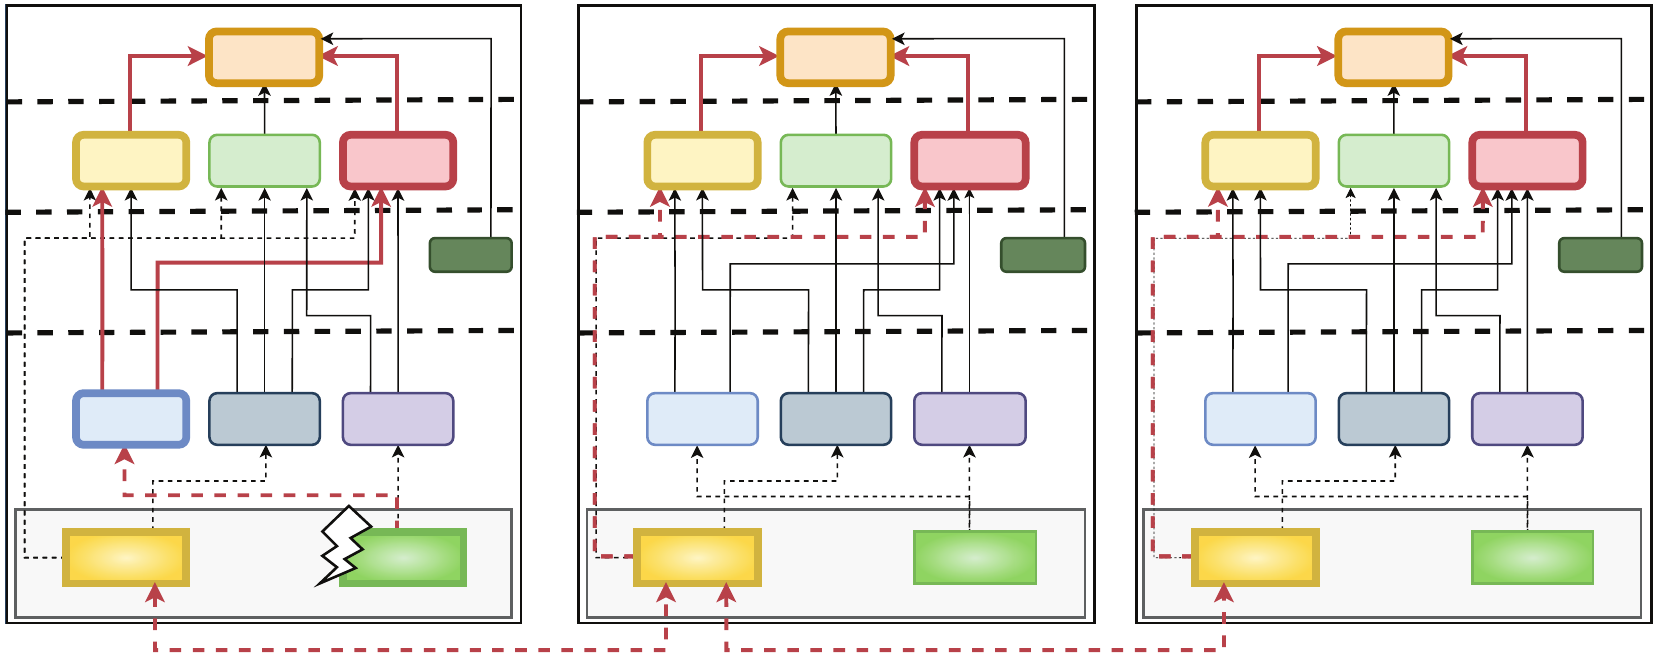
\includegraphics[width=\textwidth]{figures/gradient-dependencies-distributed.png}
        \caption{Distributed view (with neighbor dependencies).}
        \label{fig:gradient-dependencies-distributed}
    \end{subfigure}
    \caption{Dependencies between sub-computations in gradient program (\Cref{lst:gradient.scala})}
\end{figure}

\section{Design of FRASP}

% talk about constructs and semantics

\section{Design of Collektive}

% talk about constructs and semantics

\section{Integration of FRASP in Collektive}